There are two types of calculus - integral calculus, and differential calculus. This subsection will cover differential calculus, which is all centered around derivatives.

\subsection{Definition}
Derivatives are basically a souped-up version of the definition of slope that is used to find the slope at a single point of a curve.

If you start with a line, finding the slope is easy - it's rise over run, or

\begin{equation*}
    m = \frac{y_2-y_1}{x_2-x_1}
\end{equation*}

This should be familiar from Algebra I. The notation here is a little odd though - let's change it to function notation:

\begin{equation*}
    m = \frac{f(x_2) - f(x_1)}{x_2-x_1}
\end{equation*}

Let's also switch from using $f(x)$ to $f(t)$ (because often when using derivatives we're looking at how a function changes with respect to time) and treat the difference between $t_2$ and $t_1$ as $\Delta t$, or the change in $t$ ($\Delta$ as a symbol is almost always used to denote change in a quantity - it is not $\Delta * t$, but one quantity):

\begin{equation*}
    m = \frac{f(t + \Delta t) - f(t)}{\Delta t}
\end{equation*}

(Note here that we've replaced $t_2$ with $t+\Delta t$, and this makes sense because we defined $\Delta t$ as $t_2 - t_1$.) So far, this is just notational changes.

So, let's look at applying the ideas of slope to a curve. If we have two points on a curve, we can find the slope between them:

\begin{figure}[H]
    \centering
    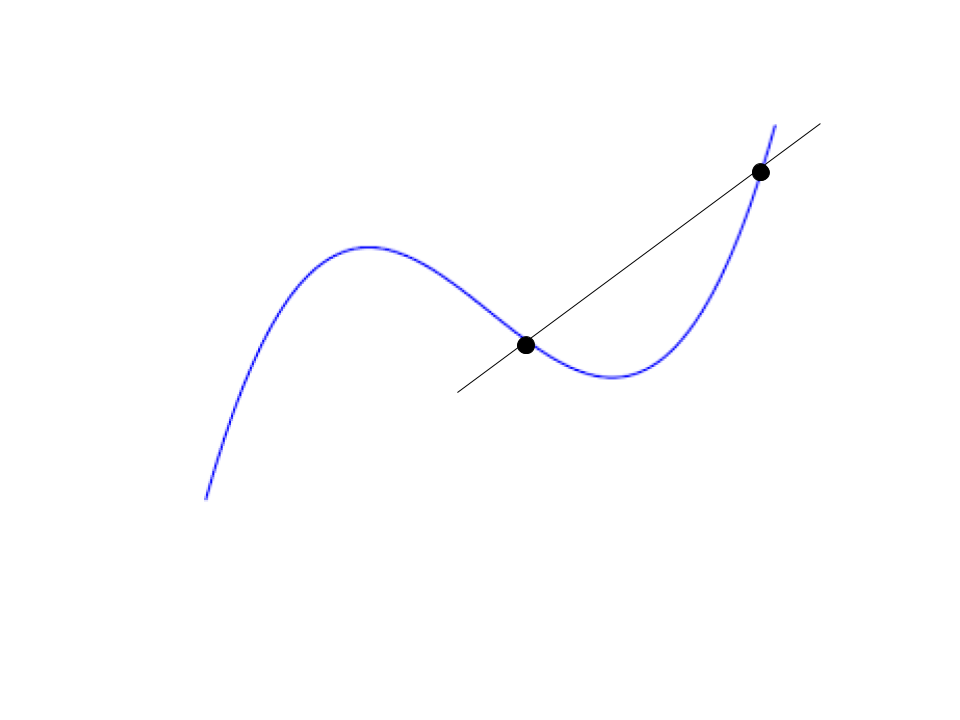
\includegraphics[scale=.15]{diagram1}
\end{figure}

But this isn't very accurate if we're trying to find the slope on, say, the descending limb of this curve. It will get more accurate if we move the two points closer:

\begin{figure}[H]
    \centering
    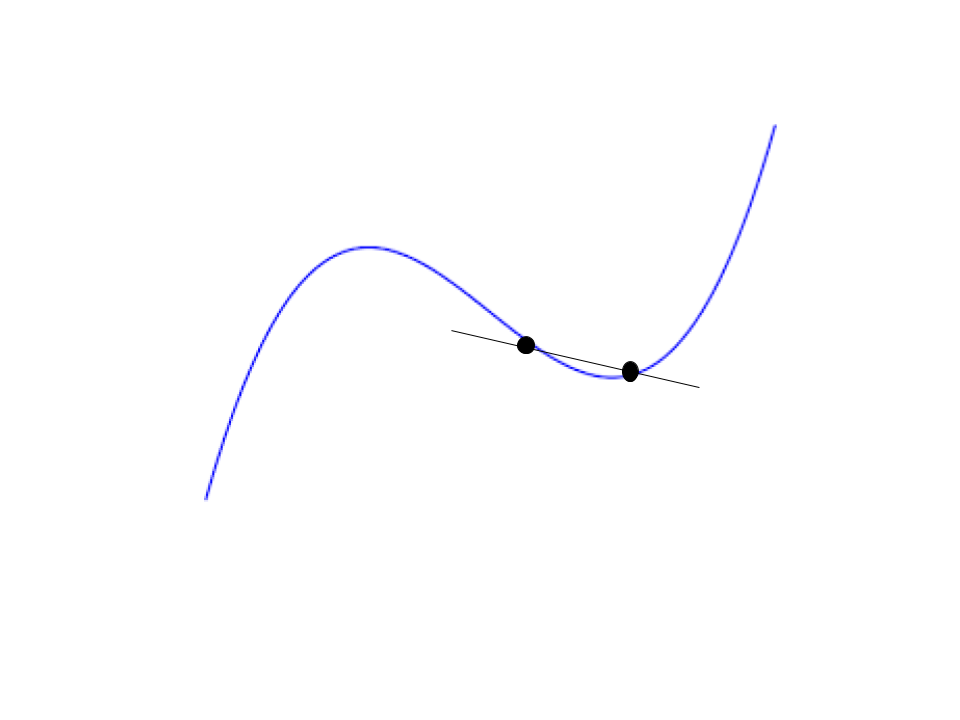
\includegraphics[scale=.15]{diagram2}
\end{figure}

And even closer:

\begin{figure}[H]
    \centering
    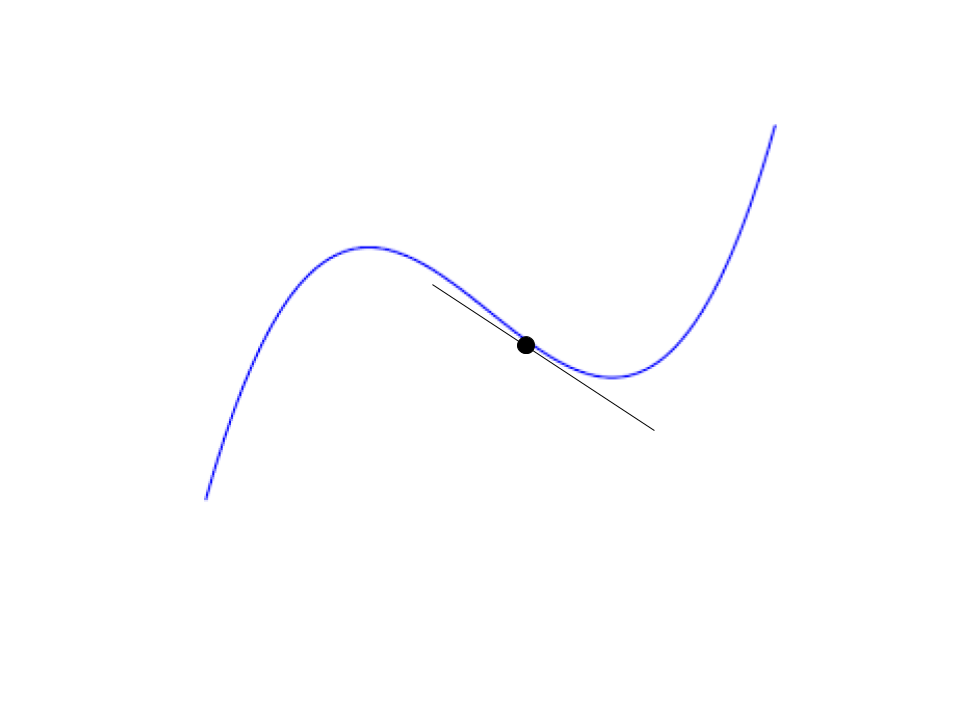
\includegraphics[scale=.15]{diagram3}
\end{figure}

Notice the distance between the points, or $\Delta t$, is approaching zero. (This is called a tangent line - a line that touches a curve at only one point. The earlier lines we drew were secant lines - lines that touch the curve at two points.) So let's add one last piece to our definition of the slope at a single point on the curve:

\begin{equation*}
    m = \lim\limits_{\Delta t\rightarrow 0} \frac{f(t+\Delta t)-f(t)}{\Delta t}
\end{equation*}

What we've added here is something called a {\it limit}. We won't go into the exact definition of a limit just yet, but for now, imagine it as a device that moves those two points closer and closer together for us. You'll probably catch a weird problem here: aren't we dividing by zero?

The answer is a little odd. Basically, we don't let $\Delta t$ approach zero until we've rearranged the equation a bit as we're calculating the derivative. We'll see this in the examples. (A quick side note - $m$ here on out is replaced by $\frac{d}{dt} f(t)$ which is read 'the derivative of $f(t)$ with respect to $t$'. The $d$ is really just a shortcut for $\Delta$, which you'll remember means the change in a particular quantity.)

\subsection{The Power Rule}

Let's do a derivative - say, the function

\begin{equation*}
    f(t) = t^2
\end{equation*}

Begin by plugging this in to our definition of a derivative:

\begin{equation*}
    \frac{d}{dt}f(t) = \lim\limits_{\Delta t\rightarrow 0}\frac{(t+\Delta t)(t+\Delta t) - t^2}{\Delta t}
\end{equation*}

This simplifies to

\begin{equation*}
    \lim\limits_{\Delta t\rightarrow 0}\frac{t^2 + 2t\Delta t + \Delta t^2 - t^2}{\Delta t}
\end{equation*}

or

\begin{equation*}
    \lim\limits_{\Delta t\rightarrow 0}\frac{2t\Delta t + \Delta t^2}{\Delta t}
\end{equation*}

or

\begin{equation*}
    \lim\limits_{\Delta t\rightarrow 0} 2t + \Delta t
\end{equation*}

Here we can now apply the limit, because there's no longer any danger of dividing by zero, and so we get

\begin{equation*}
    \frac{d}{dt}f(t) = 2t
\end{equation*}

Let's sanity check this. Look at a graph of $t^2$ - does the slope look like about $2$ at $x=1$? About $4$ at $x=2$? Remember that that's fundamentally what we're doing - looking at the slope along one section of the curve zoomed in.

That was a lot of work, and it turns out there are several rules that act as shortcuts to doing derivatives. The first of them is a power rule, and it gives the answer to the question

\begin{equation*}
    \frac{d}{dt}t^n
\end{equation*}

where $n$ is any real number. The key point here is looking at what $(t+\Delta t)^n$ looks like. Let's do the multiplication for a few numbers $n$. If $n = 2$:

\begin{equation*}
    (t+\Delta t)^2 = t^2 + 2t\Delta t + \Delta t^2
\end{equation*}

If $n = 3$:

\begin{equation*}
    (t+\Delta t)^3 = t^3 + 3t^2\Delta t + 3t\Delta t^2 + \Delta t^3
\end{equation*}

And you'll notice that if we continue with our definition of the derivative, the first term always gets canceled out by the $-f(t)$ term, and that any term with $\Delta t$ to a power greater than one becomes zero with the application of the limit (the terms with $\Delta t$ are fine because the division by $\Delta t$ cancels that bit out).

So we really know that it's the second term in the sequence that matters, and we know that term is always going to be $nt^{n-1}\Delta t$:

\begin{equation*}
    \frac{d}{dt}t^n = \lim\limits_{\Delta t\rightarrow 0} \frac{t^n + nt^{n-1}\Delta t + ... + \Delta t^n - t^n}{\Delta t}
\end{equation*}

which becomes

\begin{equation*}
    \frac{d}{dt}t^n = \lim\limits_{\Delta t\rightarrow 0} \frac{nt^{n-1}\Delta t}{\Delta t}
\end{equation*}

or

\begin{equation*}
    \frac{d}{dt}t^n = nt^{n-1}
\end{equation*}

which is the power rule for derivatives. (Note: the name for how we worked out $(t+\Delta t)^n$ is the 'binomial theorem'.)

\subsection{Product Rule}

Imagine we have a function like $f(x) = \sin(x)\cos(x)$ or something like that - something that can be rewritten as $f(x) = u(x)g(x)$ (i.e., the product of two functions) - and we want to take the derivative of it. How do we do that? (Try to take a stab at it by finding first the derivative of, e.g, $t^3$, and then the derivatives of, e.g, $t^2$ and $t$. How must they be combined to get them to equal each other?)

Let's plug this in to the formal definition:

\begin{equation*}
    \frac{d}{dt}f(x) = \lim\limits_{\Delta t\rightarrow 0} \frac{u(t+\Delta t)g(t+\Delta t)-u(t)g(t)}{\Delta t}
\end{equation*}

We have to do something that separates $g(t)$ and $u(t)$ out from each other. Maybe we can do something involving factoring - in which case we need to add some terms:

\begin{equation*}
    \frac{d}{dt}f(x) = \lim\limits_{\Delta t\rightarrow 0}\frac{u(t+\Delta t)g(t+\Delta t)-u(t+\Delta t)g(t) + u(t+\Delta t)(g(t)-g(t)u(t)}{\Delta t}
\end{equation*}

The two new terms we've added just add up to zero, but then we can factor:

\begin{equation*}
    \frac{d}{dt}f(x) = \lim\limits_{\Delta t\rightarrow 0}u(t+\Delta t)\frac{g(t+\Delta t)-g(t)}{\Delta t} + g(t)\frac{u(t+\Delta t)-u(t)}{\Delta t}
\end{equation*}

Note that two of these subsections are just the definition of the derivative:

\begin{equation*}
    \frac{d}{dt}f(x) = \lim\limits_{\Delta t\rightarrow 0} u(t+\Delta t)\frac{d}{dt}g(t)+g(t)\frac{d}{dt}u(t)
\end{equation*}

The only thing that's left is applying the limit, which gets rid of the $\Delta t$ in the first term:

\begin{equation*}
    \frac{d}{dt}f(x) = u(t)\frac{d}{dt}g(t)+g(t)\frac{d}{dt}u(t)
\end{equation*}

And this is the product rule.

\subsection{Chain Rule}

The chain rule deals with cases where you want to differentiate a function like $f(x) = (5x)^2$ - that is, functions that can be rewritten as $f(x) = g(u(x))$.

The chain rule is kind of intuitive in some ways - it's a lot like what we do for unit conversions. Imagine we were doing a unit conversion from seconds to minutes of a quantity $c$. Then we might do $c\times\frac{1\text{ minute}}{60\text{ seconds}}$. Similarly, for the chain rule, we're switching 'units' - which thing we're differentiating with respect to:

\begin{equation*}
    \frac{d}{dx}f(x) = \frac{dg}{du}\frac{du}{dx}
\end{equation*}

That is, we're differentiating $g(u)$ with respect to $u$ (in the example above, this would be the derivative of $u^2$) and then multiplying that by the derivative of $u(x)$ with respect to $x$ (in the example above, the derivative of $5x$).

While this may not be a formal proof, the intuition here is quite useful and sufficient for now, but feel free to look up the actual proof or come up with your own.

\subsection{Quotient Rule}

The quotient rule derives fairly cleanly from the product, chain, and power rules. Say we want to take the derivative of a function $f(x) = \frac{g(x)}{u(x)}$. We can rewrite this as $f(x) = g(x)u^{-1}(x)$. Then, we use the product rule:

\begin{equation*}
    g(x)\frac{d}{dx}u^{-1}(x) + u^{-1}(x)\frac{d}{dx}g(x)
\end{equation*}

(Quick note - one can also use an apostrophe to indicate the derivative of something - e.g., $f'(x)$ or $f'$ is the derivative of f. I'll use this occasionally when it'll make something neater.) On the derivative of $u^{-1}$ we can use the chain rule and power rule:

\begin{equation*}
    g(x)(u')(-u^{-2})+u^{-1}g'
\end{equation*}

(Remember $u^{-1}$ is just another way we're writing $u$; since it's in the derivative and we can't simplify it further, we'll leave it be.) Then we can do

\begin{equation*}
    \frac{-gu'}{u^2}+\frac{g'}{u}
\end{equation*}

Finally, we get

\begin{equation*}
    \frac{d}{dx}f(x) = \frac{gf' - fg'}{g^2}
\end{equation*}

And that's the quotient rule!

\subsection{Constants and the addition rule}

These last pieces should be attempted on your own: prove that the derivative of a constant $c$ is always zero, and prove that 

\begin{equation*}
    \frac{d}{dx}\left[u(x) + g(x)\right] = \frac{d}{dx}u(x) + \frac{d}{dx}g(x)
\end{equation*}

Both of these pop right out of the definition of a derivative. (From here, too, one can easily figure out the subtraction rule for derivatives.)

\subsection{When are things not differentiable?}

A function is differentiable if you can find the derivative of it at each point in that function's domain. \textit{This isn't always possible.} Remember our original definition:
\begin{equation*}
    \frac{d}{dx}f(x) = \lim_{\Delta t\rightarrow 0} \frac{f(t+\Delta t) - f(t)}{\Delta t}
\end{equation*}
Sometimes we cannot zoom in properly on a single point (remember we said the limit effectively moves the two points on the secant line closer and closer together until it is a tangent line). For instance, take the following graphs:
\begin{figure}[H]
    \centering
    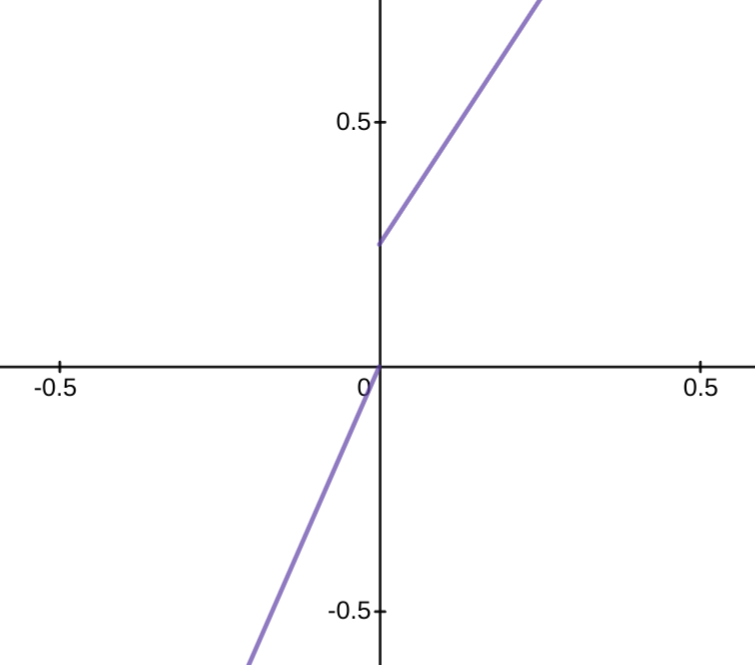
\includegraphics[scale=.1]{split.png}
    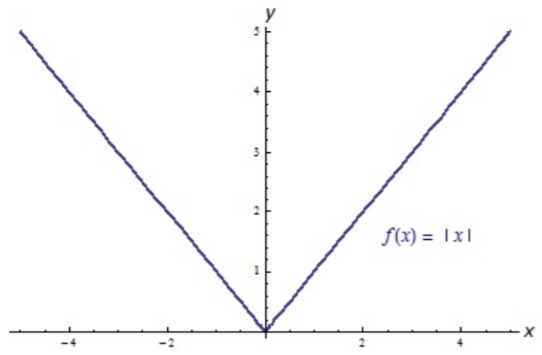
\includegraphics[scale=.15]{corner.png}
    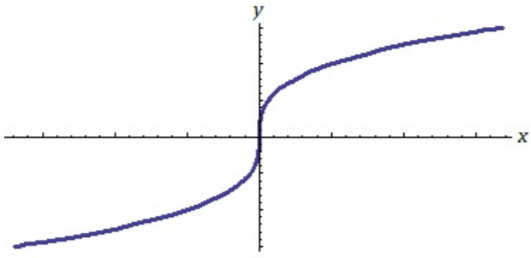
\includegraphics[scale=.2]{steep.png}
    \label{fig:my_label}
\end{figure}

Looking at the first graph, notice that if we tried to take the derivative at zero, we wouldn't be able to have a single tangent line - just looking at the top portion of the graph, it seems like the slope at zero should be 2 or so, but looking at the top portion, it seems like the slope should be 3 or so. There is a disconnect (more formally, the graph isn't continuous) and so we can't find the derivative. (In section 4.3.2, this turns out to be formalized by saying the limits from the left and right aren't equal.)

Looking at the second graph, there's a somewhat similar issue. There's a sharp corner, not a smooth change, which means that as we approach from the left side of the graph, the slope/derivative seems like it should be -1 at zero, whereas from the right side of the graph, it seems like it should be 1. These aren't equal, and we can't find the derivative at that point.

Finally, looking at the third graph, we have a slightly different problem. It's easy to draw a tangent line at zero...but it's vertical. The slope can be best described as infinity, maybe, but it's not something that could be cleaned up if we tried to plug it into our definition of the derivative.

So we can roughly categorize the things we can't take derivatives of as having jumps, corners, or vertical asymptotes.